% !TeX root = Trafficsimulation_Documentation.tex

\chapter{Design}
\label{Design}

In diesem Kapitel werden die Implementierungen der einzelnen Komponenten sowie deren Schnittstellen zu anderen Komponenten dokumentiert.

\thispagestyle{standard}
\pagestyle{standard}

\section{Strassensystem}
\label{Strassensystem}

\subsection{Ampeln}

Die Ampeln wurden von uns als eigenständiges System geplant und umgesetzt. Um dieses Ziel zu erreichen erstellten wir zuerst auf Basis der Technologie TCP-Channel ein RemoteObject in Form einer eigenen DLL. Dieses RemoteObject definiert die Datenstrukturen, welche in weiterer Folge zwischen Client und Server geteilt werden. Als Serveranwendung erstellten wir eine Konsolenanwendung, welche wir auf einem öffentlich erreichbaren Linux Server mit Hilfe von Mono deployten. Als Clientgegenstellen für dieses System können verschiedene Unityinstanzen den Dienst der Serveranwendung verwenden. Sowohl am Client als auch am Server ist als DLL das RemoteObject hinterlegt. Instanzen des RemoteObjects können mit Hilfe am Server definierten Interfaces von den Clients erstellt und bearbeitet werden. Die somit erstellten Instanzen werden dann durch die TCP-Channel Technologie zwischen Client unser Server geteilt. Somit können Clients komfortabel mit ihrem lokalen Stub des RemoteObjects arbeiten ohne die Komplexität der IPC mitzubekommen. 

Durch die zentrale Definition des RemoteObjects in Form einer DLL können die geteilten Datenstrukturen zentral erweitert und gewartet werden.

\subsection{Strassen}

\subsection{Kreuzungen}

\section{Fahrzeuglogik}
\label{Fahrzeuglogik}

\section{Ampelsteuerung}

Die zentrale Komponente der Ampelsteuerung ist das RemoteObject. Wie bereits erwähnt handelt es sich dabei um eine eigenständige Komponente, welche in Form einer DLL in diverse Projekte leicht eingebunden und zentral gewartet werden kann. Das RemoteObject repräsentiert die Datenstrukturen und Funktionalitäten, welche zwischen Client und Server mit Hilfe der TCP-Channel Technologie geteilt werden.

Das RemoteObject bietet die Möglichkeit eine beliebige Anzahl von Kreuzungen zu erstellen und zu verwalten. Die Logik für den Aufbau der IPC-Verbindung wird dabei direkt im Client oder Server hinterlegt. Mit Hilfe von definierte Interfaces hat der Client die Möglichkeit Kreuzungen mit drei oder vier Ampeln am Server-Skeleton anzulegen. Die Kreuzungen werden entweder mit einer festgelegten Standardkonfiguration oder mit den vom Entwickler angegeben Übergabeparametern angelegt.

Von bereits angelegten Kreuzungen können die Zykluszeiten der einzelnen Ampeln editiert werden. Weiters ist es möglich das RemoteObject zu reseten und somit den Initialzustand wiederherzustellen.

Die einzelnen Kreuzungen, welche am RemoteObject angelegt sind können separat gestartet werden. Beim Starten einer Kreuzung wird ein eigener Thread für jede Ampel der Kreuzung erzeugt in dem eine Statemachine für die Ampelschaltung abläuft. Dieser Thread läuft bis entweder die Serveranwendung terminiert wird oder die Kreuzung durch einen Reset vom Client gelöscht wird. Die Statemachine einer Ampel durchläuft die üblichen Stati und berücksichtigt dabei die Konfiguration der entsprechenden Ampel. 

Mit Hilfe der ID einer Kreuzung und der Bezeichnung einer konkreten Ampel der Kreuzung kann der Status einer Ampel abgefragt werden.

Durch die Verwendung der TCP-Channel Technologie und der Definition des RemoteObjects in Form einer eigenen DLL wurde die Komplexität einer IPC sehr gut abstrahiert. Leider erfuhren wir während den Tests, dass die von uns verwendete Technologie sehr anfällig gegenüber schlechten Latenzzeiten ist. Dies wirkt sich in Form von Verbindungsproblemen zwischen Client und Server aus. Daher würde ich die Technologie TCP-Channel für IPC nur innerhalb eines lokalen Netzwerkes empfehlen.


\section{Hindernisse}
\label{Hindernisse}

Mit einem Klick der Maus sollen überall in der Welt Hindernisse platziert werden, welche anschließend von Fahrzeugen umfahren werden müssen. Durch einen weiteren Klick auf ein Hindernis soll dieses wieder gelöscht werden. 

Unity ermöglicht das Erstellen von GameObjects zur Laufzeit. Durch den Klick auf die Welt können die Koordinaten des Klicks festgestellt werden und somit das GameObject, welches bereits beim Start der Verkehrssimulation geladen wurde, platziert werden.

Durch das Halten eines Buttons auf der Tastatur soll die Erstellung von Hindernissen aktiviert werden. Dies verhindert, dass der Benutzer unbeabsichtigt zu viele Hindernisse erstellt.

\section{Aus- und Einfahren von Fahrzeugen anderer Gruppen}

Mit dem Plugin `Unity3D.Amqp` (\url{https://github.com/CymaticLabs/Unity3D.Amqp}) für Unity ist es möglich einen RabbitMQ-Server direkt in Unity einzubinden.

Die Konfiguration der Serverdaten werden dabei direkt in den Menüeinstellungen von Unity vorgenommen. Die verwendete Konfiguration ist in Abbildung \ref{img:rabbit} zu sehen.

\begin{figure}[H]
\begin{center}
	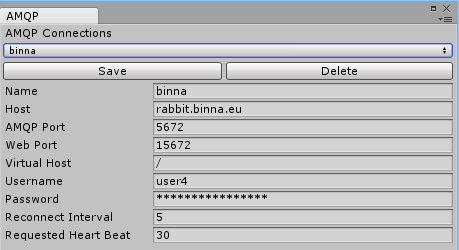
\includegraphics[width=0.9\textwidth]{BilderAllgemein/rabbitconfig.png}
\end{center}

	\caption{Einstellungen RabbitMQ}

	\label{img:rabbit}
\end{figure}

Jede Gruppe bekam einen eigenen Benutzer samt Passwort. Damit man Nachrichten empfangen kann, muss man sich auf eine `Queue` subscriben.

Das Plugin stellt anschließend Methoden zur Verfügung. Eine solche Methode ist \texttt{OnMessageReceived()}. Damit lässt sich eine eingehende Nachricht an ein Objekt in der Spielwelt weitergeben. Das Objekt kann daraufhin reagieren, beispielsweise ein Auto erzeugen.

\begin{figure}[H]
\begin{center}
	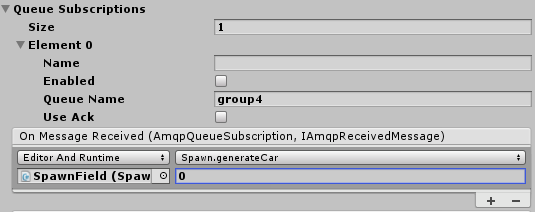
\includegraphics[width=0.9\textwidth]{BilderAllgemein/rabbitqueue.png}
\end{center}

	\caption{RabbitMQ Queue}

	\label{img:rabbitq}
\end{figure}

In Abbildung \ref{img:rabbitq} sieht man wie eine eingehende Nachricht beim Objekt \texttt{SpawnField} eine Methode aufruft.